\expandafter\newcommand\csname Slidep01\endcsname{%
\renewcommand{\defenseblock}{Introducción}
\renewcommand{\defensenav}{Defensa del TFG}
\begin{frame}[plain]\hypertarget{p01}{}
\centering
\vspace*{5mm}

\includegraphics[height=33mm]{assets/logo_uniovi_portada.pdf}\par
\vspace{6mm}
{\fontsize{32}{40}\selectfont\ThesisTitle\par}
\vspace{7mm}
{\fontsize{19}{25}\selectfont\DegreeName\par}
\vspace{6mm}
{\fontsize{21}{27}\selectfont\AuthorName\par}
{\fontsize{17}{23}\selectfont Tutor: \SupervisorName\par}
\vfill

\includegraphics[height=9mm]{assets/logo_epi_horizontal.pdf}\hfill
{\fontsize{17}{22}\selectfont\SubmissionDate}\par
\note{Buenos días. Este TFG estudia la clasificación de imágenes de ECG con pocos ejemplos etiquetados y utiliza el síndrome de Brugada como caso de estudio.}
\end{frame}}

\expandafter\newcommand\csname Slideproblema\endcsname{%
\renewcommand{\defenseblock}{Introducción}
\renewcommand{\defensenav}{Defensa del TFG}
\begin{frame}[t]\hypertarget{problema}{}
\frametitle{Enfermedades cardiovasculares y síndrome de Brugada}
\vspace{7mm}
\begin{columns}[c,onlytextwidth]
\begin{column}{.56\textwidth}
\centering
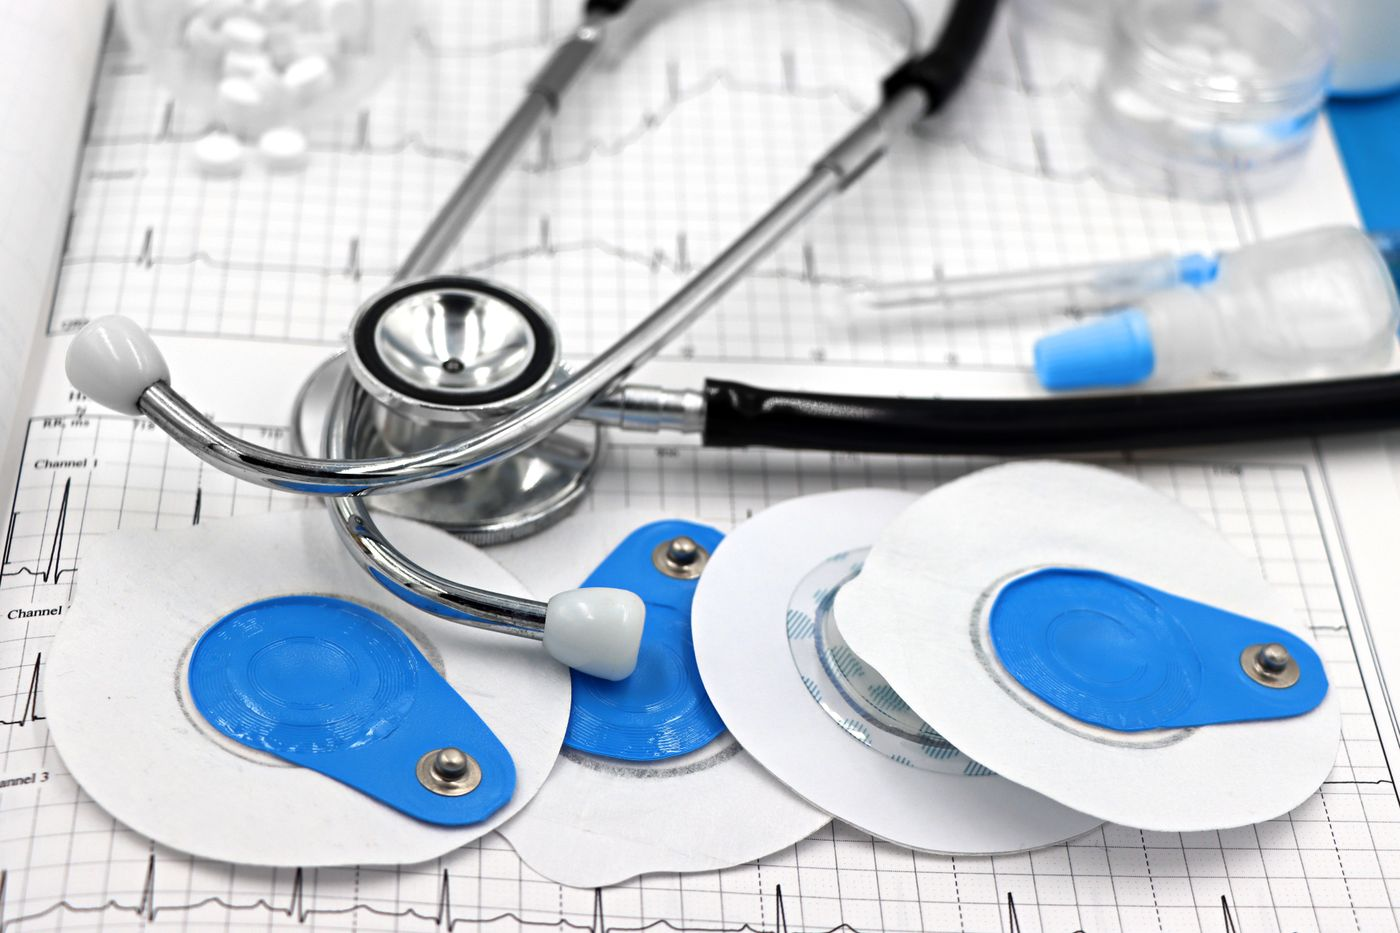
\includegraphics[width=\linewidth,height=103mm,keepaspectratio]{assets/referencias_visuales/electrodos.jpg}\par
\credit{\href{https://www.pexels.com/photo/medical-instruments-on-electrocardiogram-printout-35044386/}{Fotografía de Marta Branco, Pexels.}}
\end{column}
\begin{column}{.39\textwidth}
{\color{UOGreen}\fontsize{42}{49}\selectfont 19,8 millones\par}
\vspace{2mm}
{\fontsize{19}{25}\selectfont de muertes cardiovasculares\\en el mundo en 2022.\par}
\credit{\href{https://www.who.int/en/news-room/fact-sheets/detail/cardiovascular-diseases-(cvds)}{Estimación de la OMS.}}
\vspace{8mm}
{\color{UOGreen}\fontsize{23}{30}\selectfont Síndrome de Brugada\par}
{\fontsize{19}{25}\selectfont Una enfermedad poco frecuente\\con pocos ECG etiquetados.\par}
\end{column}
\end{columns}
\note{Según la OMS, las enfermedades cardiovasculares causaron unos 19,8 millones de muertes en el mundo en 2022. Dentro de este grupo hay trastornos poco frecuentes, como el síndrome de Brugada. En Brugada cuesta reunir suficientes ECG etiquetados. El TFG explora cómo aprovecharlos para una futura herramienta de apoyo al triaje.}
\end{frame}}

\expandafter\newcommand\csname Slidep02\endcsname{%
\renewcommand{\defenseblock}{Introducción}
\renewcommand{\defensenav}{Defensa del TFG}
\begin{frame}[plain]\hypertarget{p02}{}
\begin{tikzpicture}[remember picture,overlay,x=1mm,y=-1mm]
\begin{scope}[shift={(current page.north west)}]
\node[anchor=north west,inner sep=0pt] at (0,0)
  {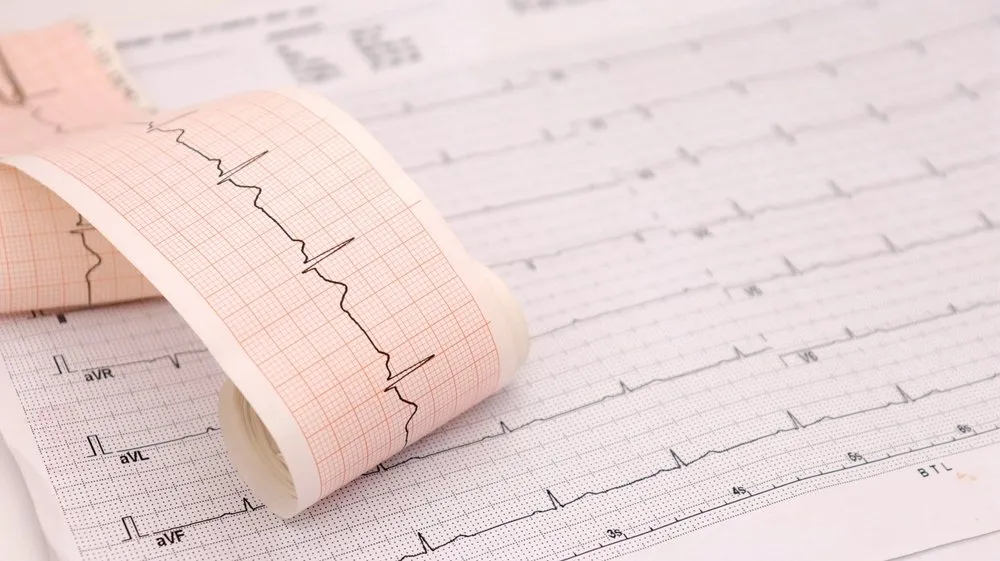
\includegraphics[viewport=0 86 1000 445,clip,width=\paperwidth]{assets/referencias_visuales/electrocardiograma_papel_adjunto.png}};
\node[anchor=north west,inner sep=0pt,text=UOInk] at (16,120)
  {\fontsize{40}{47}\selectfont Electrocardiograma en formato imagen};
\node[anchor=north west,inner sep=0pt,text=UOGreen] at (16,145)
  {\fontsize{21}{28}\selectfont Si solo tenemos el trazado, podemos analizarlo directamente como imagen.};
\node[anchor=south east,inner sep=0pt,text=UOGray] at (302,172)
  {\fontsize{11}{14}\selectfont\insertframenumber};
\end{scope}
\end{tikzpicture}
\note{Esta fotografía muestra una forma en que puede conservarse o compartirse un ECG. En algunos registros solo está disponible el trazado impreso o su copia como imagen. Para analizarlo, una opción es reconstruir la serie temporal. Aquí estudiamos la clasificación directa a partir de imágenes del trazado. En el experimento, la entrada de ambos modelos es la imagen de un latido de V1.}
\end{frame}}

\expandafter\newcommand\csname Slideobjetivos\endcsname{%
\renewcommand{\defenseblock}{Introducción}
\renewcommand{\defensenav}{Defensa del TFG}
\begin{frame}[t]\hypertarget{objetivos}{}
\frametitle{Propuesta y objetivos del TFG}
\vspace{5mm}
{\fontsize{20}{27}\selectfont\color{UOGreen} Apoyar el triaje de ECG sospechosos.\par}
\vspace{8mm}
{\fontsize{25}{34}\selectfont
{\color{UOGreen}01}\quad Efecto del número de ejemplos de entrenamiento o de contexto\par\vspace{10mm}
{\color{UOGreen}02}\quad Comparación entre una CNN supervisada y un VLM con ICL\par\vspace{10mm}
{\color{UOGreen}03}\quad Transferencia de datos sintéticos a datos clínicos\par}
\note{El TFG explora cómo apoyar el triaje de ECG sospechosos. En el análisis de ECG, este TFG estudia tres preguntas. ¿Cómo varía el rendimiento cuando se dispone de más ejemplos, ya sea para entrenar la red o para construir el contexto? ¿Cómo se compara una red convolucional supervisada con un modelo de visión y lenguaje que aprende en contexto? ¿En qué medida se conserva el rendimiento al pasar de ejemplos sintéticos a registros clínicos?}
\end{frame}}

\expandafter\newcommand\csname Slideindice\endcsname{%
\renewcommand{\defenseblock}{Introducción}
\renewcommand{\defensenav}{Defensa del TFG}
\begin{frame}[t]\hypertarget{indice}{}
\frametitle{Estructura de la exposición}
\vspace{8mm}
{\fontsize{25}{34}\selectfont
\hyperlink{antecedentes}{1. Estado del arte y fundamentos}\par\vspace{7mm}
\hyperlink{p05}{2. Datos, simulación e implementación}\par\vspace{7mm}
\hyperlink{escenarios}{3. Escenarios y protocolo de evaluación}\par\vspace{7mm}
\hyperlink{escenario_simulador}{4. Resultados en los tres escenarios}\par\vspace{7mm}
\hyperlink{p15}{5. Discusión, conclusiones y continuación}\par}
\note{Primero situaré el trabajo y explicaré sus fundamentos. Después presentaré los datos, el simulador y los modelos. Antes de los resultados veremos los tres escenarios y cómo se evalúa cada paciente.}
\end{frame}}

\expandafter\newcommand\csname Slideantecedentes\endcsname{%
\renewcommand{\defenseblock}{Introducción}
\renewcommand{\defensenav}{Defensa del TFG}
\begin{frame}[t]\hypertarget{antecedentes}{}
\frametitle{Estado del arte}
\begin{columns}[c,onlytextwidth]
\begin{column}{.49\textwidth}
\centering
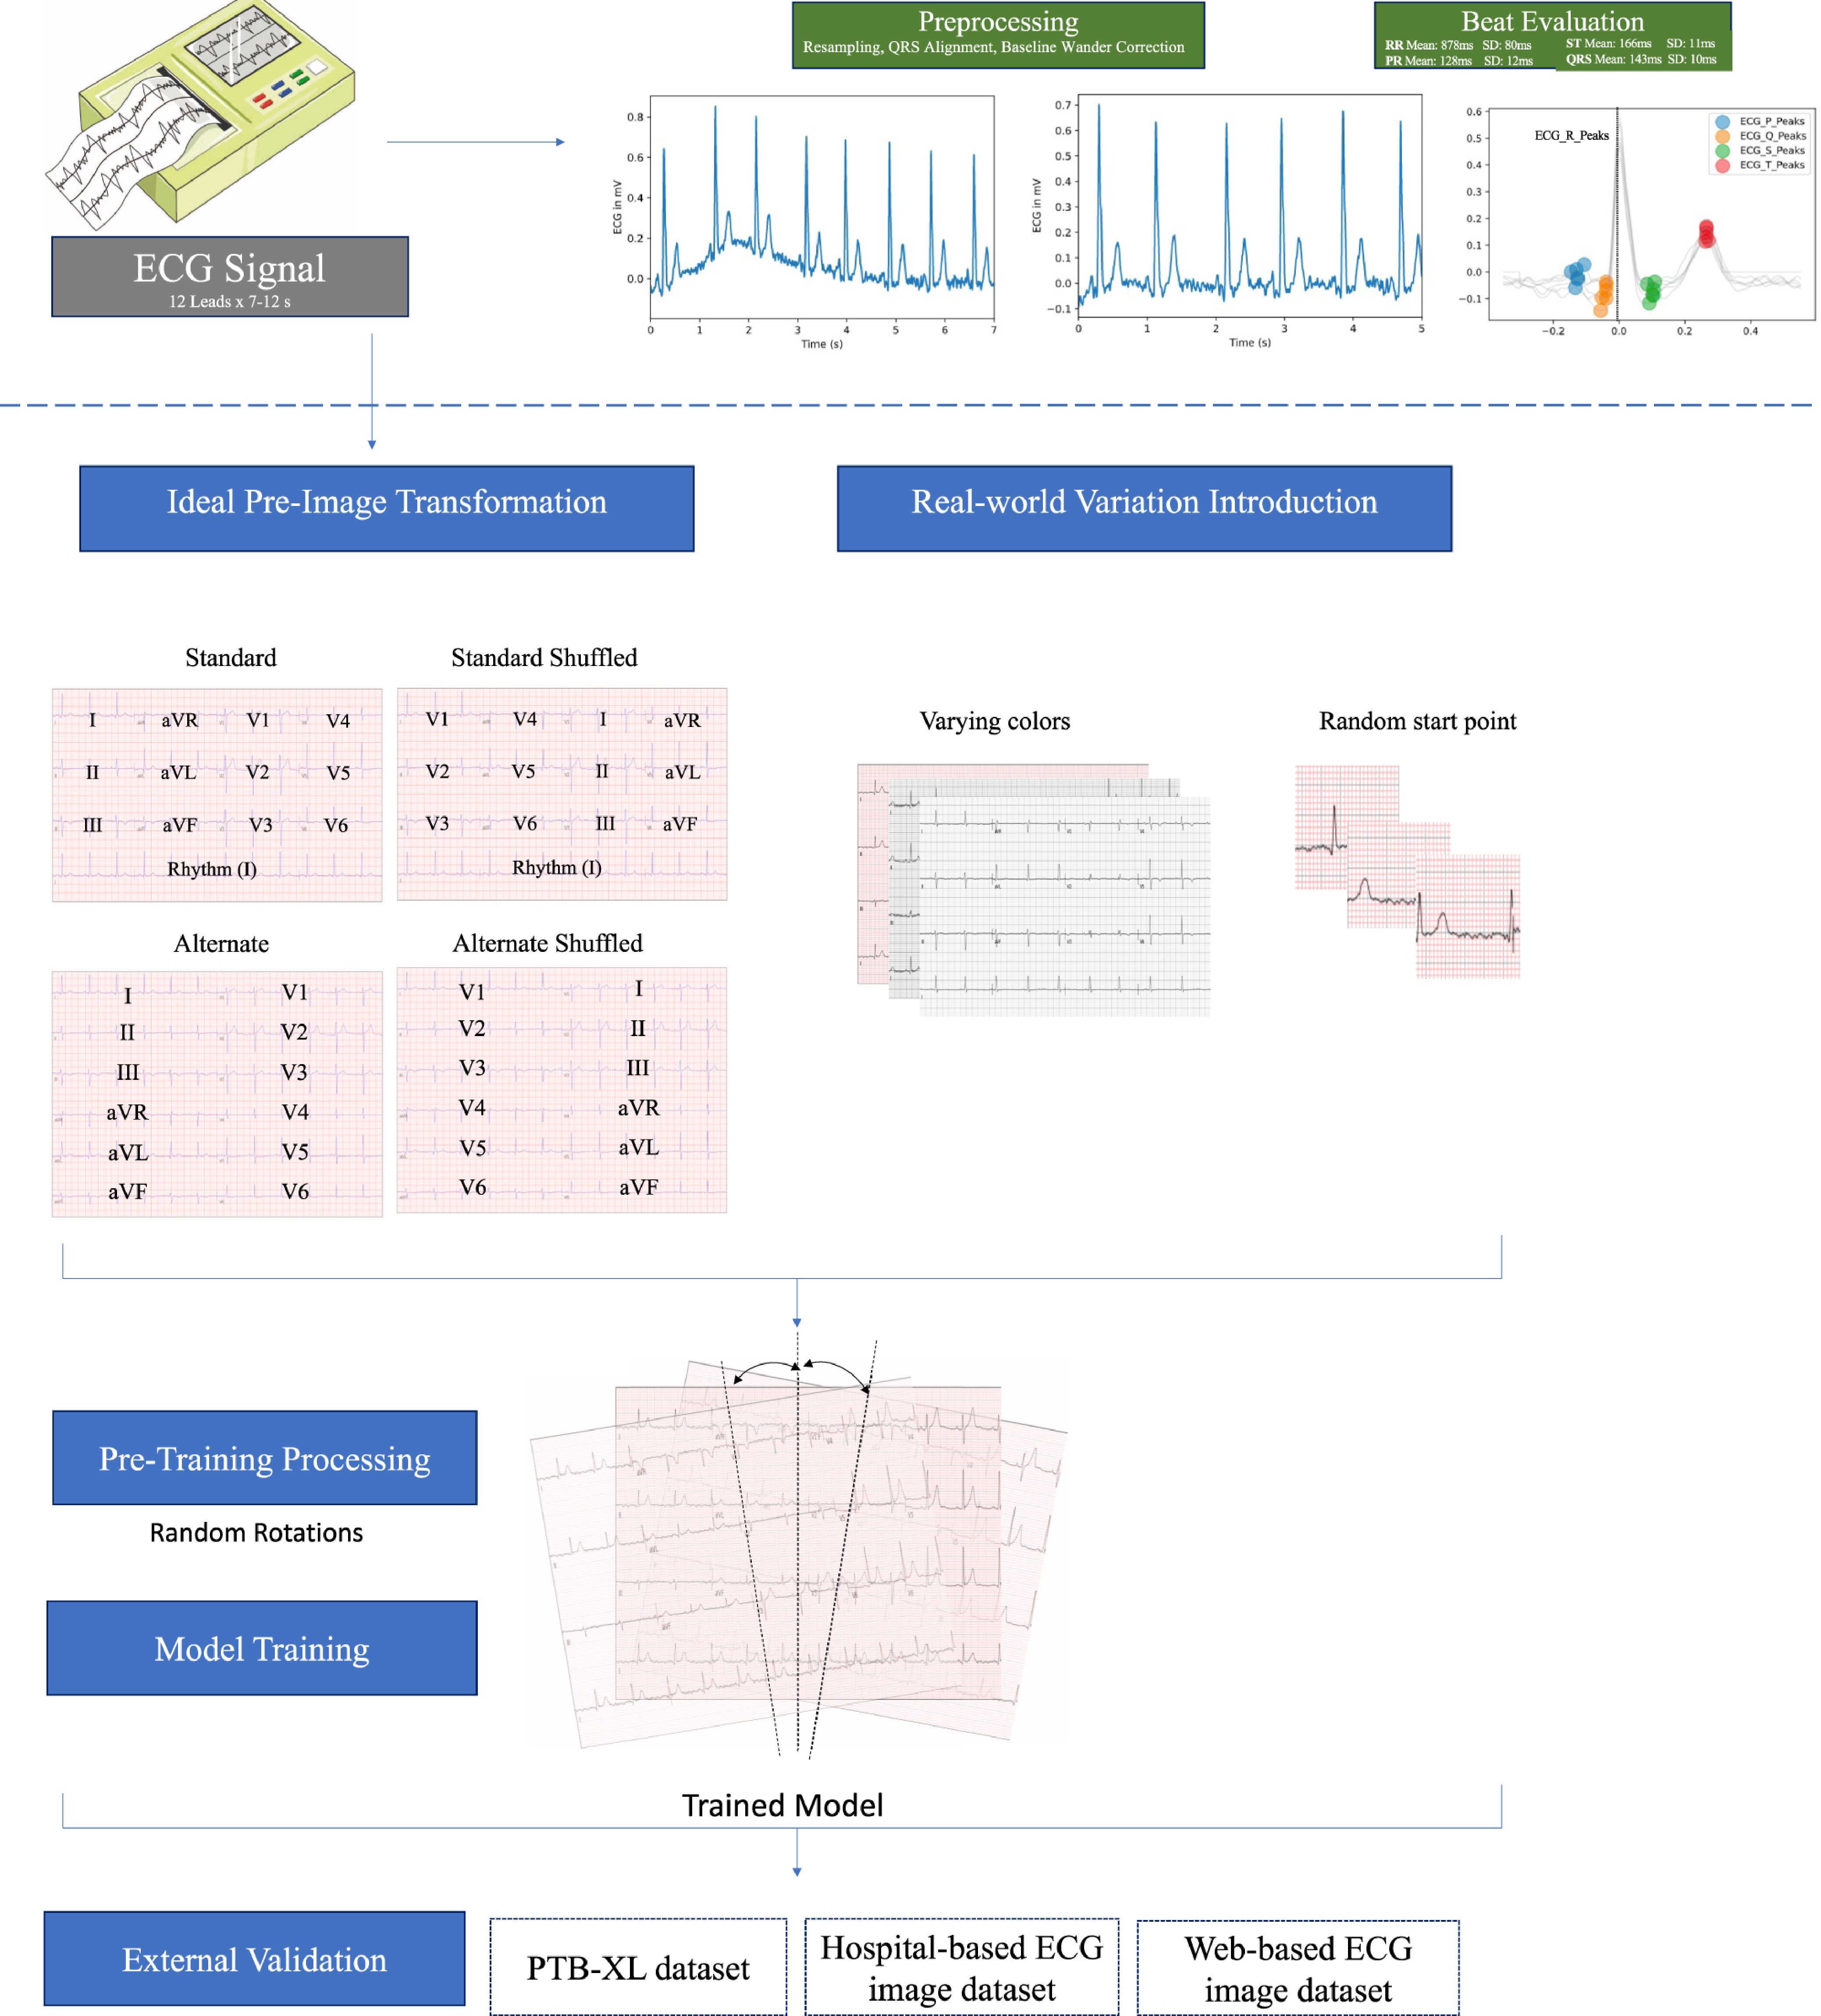
\includegraphics[trim=0 735bp 0 0,clip,width=\linewidth,height=110mm,keepaspectratio]{assets/referencias_visuales/sangha.pdf}\par
\end{column}
\begin{column}{.46\textwidth}
{\color{UOGreen}\fontsize{24}{30}\selectfont ECG como señal\par}
{\fontsize{19}{26}\selectfont Ribeiro et al. (2020)\par}
\vspace{6mm}
{\color{UOGreen}\fontsize{24}{30}\selectfont ECG como imagen\par}
{\fontsize{19}{26}\selectfont Sangha et al. (2022)\par}
\vspace{6mm}
{\color{UOGreen}\fontsize{24}{30}\selectfont Aprendizaje en contexto\par}
{\fontsize{19}{26}\selectfont Ejemplos etiquetados en la consulta.\par}
\end{column}
\end{columns}
\note{Ribeiro y colaboradores estudiaron la clasificación de señales de ECG con registros de la red de telemedicina de Minas Gerais. Sangha y colaboradores entrenaron con registros brasileños convertidos en imágenes y realizaron una validación externa que incluyó PTB-XL. Camba y Costa estudiaron métodos con pocos ejemplos en ECG. Con ICL, los ejemplos etiquetados se incorporan directamente a la consulta.}
\end{frame}}

\expandafter\newcommand\csname Slidelatido\endcsname{%
\renewcommand{\defenseblock}{Fundamentos clínicos}
\renewcommand{\defensenav}{Defensa del TFG}
\begin{frame}[t]\hypertarget{latido}{}
\frametitle{Cómo leer un latido}
\centering
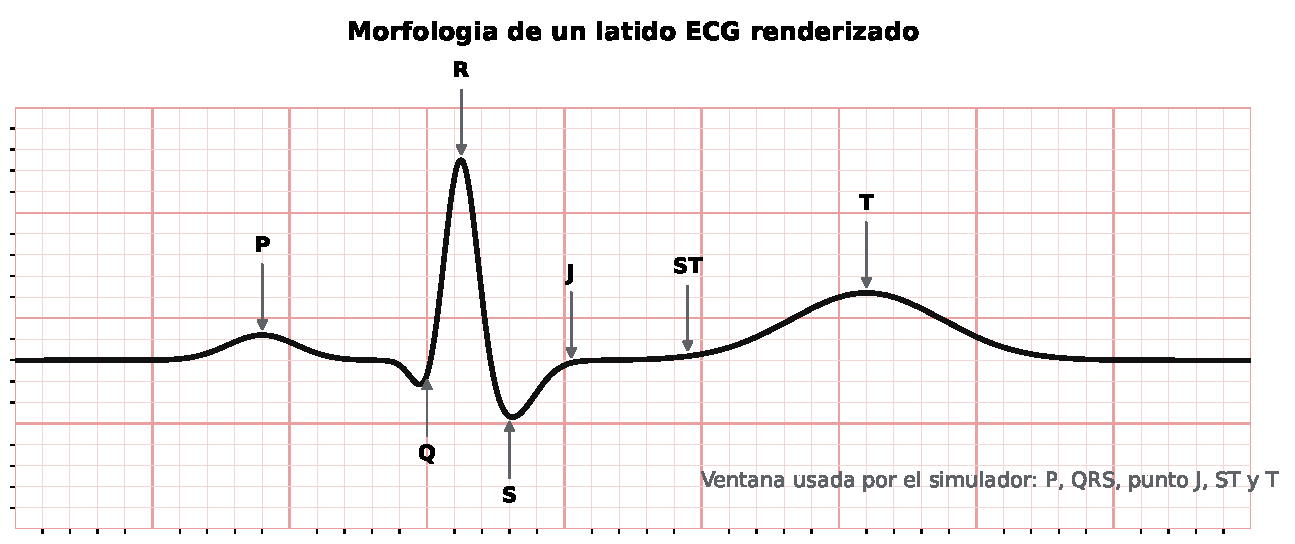
\includegraphics[trim=3bp 4bp 2bp 25bp,clip,width=226mm]{assets/fig_morfologia_ecg.pdf}\par
\vspace{4mm}
\begin{columns}[T,onlytextwidth]
\begin{column}{.34\textwidth}
{\color{UOGreen}\fontsize{20}{26}\selectfont Complejo QRS\par}
{\fontsize{16}{22}\selectfont Activación ventricular. El RBBB es un bloqueo de rama derecha que cambia la parte final del QRS.\par}
\end{column}
\begin{column}{.30\textwidth}
{\color{UOGreen}\fontsize{20}{26}\selectfont Segmento ST\par}
{\fontsize{16}{22}\selectfont Empieza en el punto J. Se observa si está elevado respecto a la línea de base.\par}
\end{column}
\begin{column}{.28\textwidth}
{\color{UOGreen}\fontsize{20}{26}\selectfont Onda T\par}
{\fontsize{16}{22}\selectfont Repolarización ventricular. Se observa si la onda está invertida.\par}
\end{column}
\end{columns}
\note{Leemos el trazado de izquierda a derecha. La P corresponde a la activación de las aurículas y el QRS, a la de los ventrículos. En el bloqueo de rama derecha, o RBBB, el ventrículo derecho se activa con retraso y puede aparecer una segunda deflexión positiva al final del QRS. En el simulador, RBBB etiqueta ese rasgo morfológico. Después del punto J miramos si el ST se eleva respecto a la línea de base y si la onda T, que corresponde a la repolarización ventricular, apunta hacia abajo.}
\end{frame}}

\expandafter\newcommand\csname Slidep03\endcsname{%
\renewcommand{\defenseblock}{Fundamentos clínicos}
\renewcommand{\defensenav}{Defensa del TFG}
\begin{frame}[t]\hypertarget{p03}{}
\frametitle{Síndrome de Brugada y derivación V1}
\begin{columns}[c,onlytextwidth]
\begin{column}{.55\textwidth}
\centering
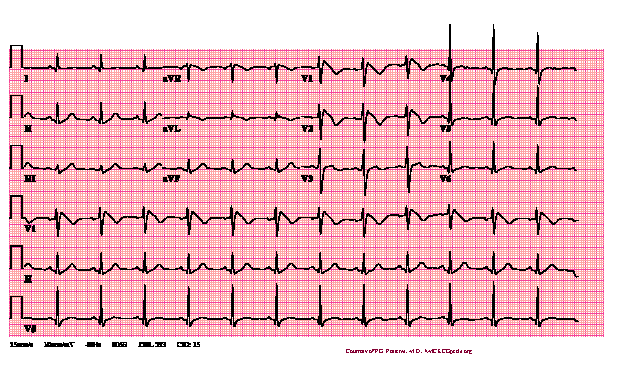
\includegraphics[trim=3bp 4bp 5bp 9bp,clip,width=\linewidth,height=108mm,keepaspectratio]{assets/brugada_type1_ecgpedia.pdf}
\end{column}
\begin{column}{.43\textwidth}
\centering
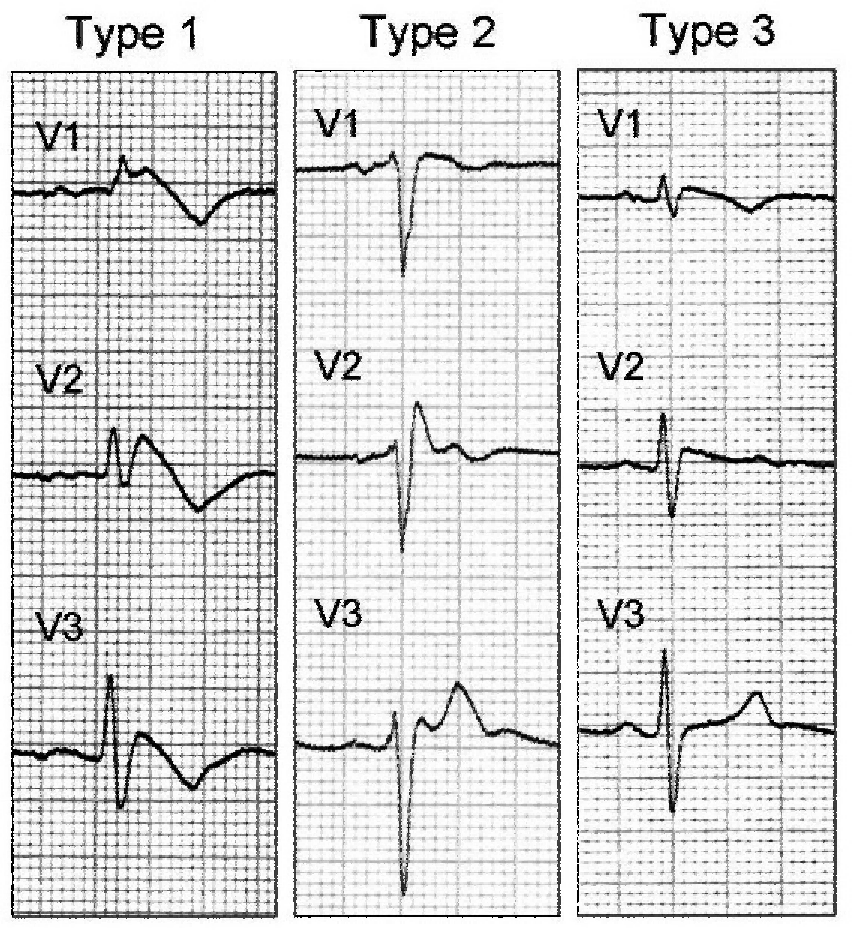
\includegraphics[width=\linewidth,height=101mm,keepaspectratio]{assets/brugada_patterns_orphanet.pdf}
\end{column}
\end{columns}
\centering
{\fontsize{18}{24}\selectfont QRS terminal \enspace\textperiodcentered\enspace Elevación del ST \enspace\textperiodcentered\enspace Onda T negativa\par}
\credit{Izquierda: ECGpedia / CardioNetworks, CC BY-SA 3.0. Derecha: Napolitano y Priori (2006), CC BY 2.0.}
\note{V1 es una derivación precordial derecha. En estos ejemplos, fijaos en cómo termina el QRS y cómo continúa el trazado. En el patrón de Brugada tipo 1, el ST desciende desde un punto elevado y le sigue una onda T negativa. El simulador modifica de forma controlada la parte terminal del QRS, el ST y la onda T.}
\end{frame}}

\expandafter\newcommand\csname Slidecnn_concepto\endcsname{%
\renewcommand{\defenseblock}{Fundamentos metodológicos}
\renewcommand{\defensenav}{Defensa del TFG}
\begin{frame}[t]\hypertarget{cnn_concepto}{}
\frametitle{Redes neuronales convolucionales}
\centering
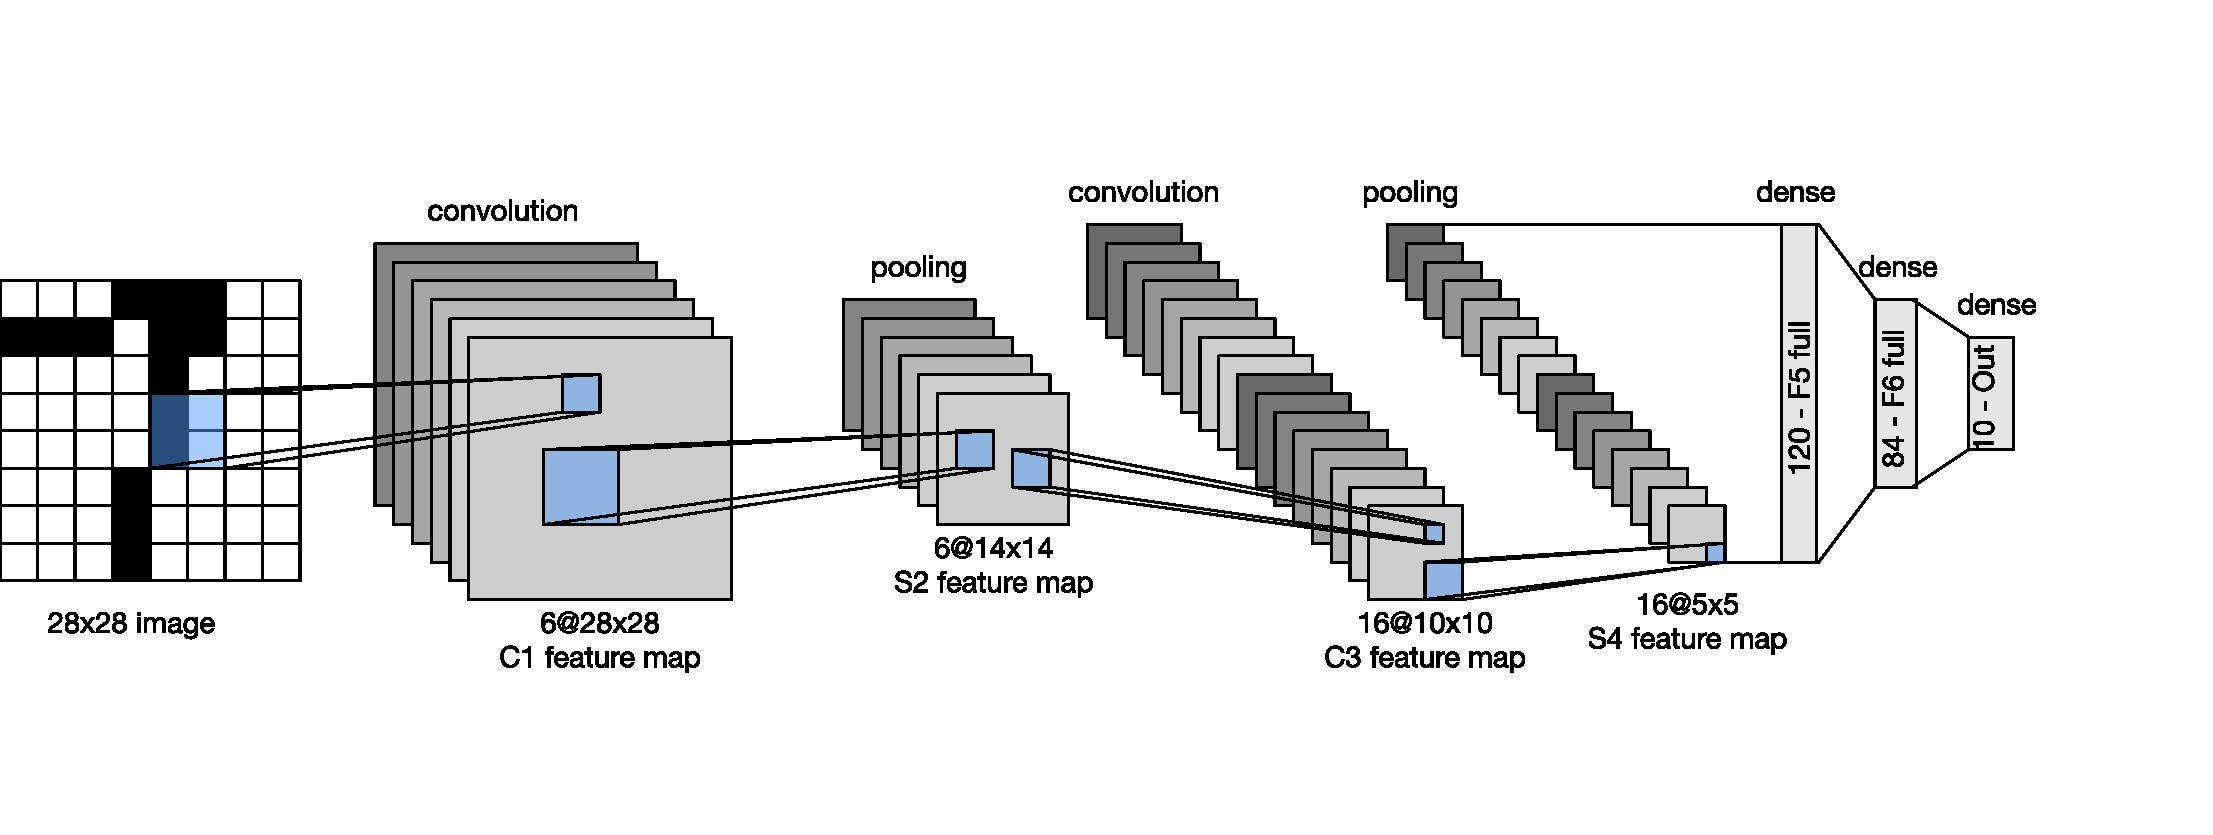
\includegraphics[trim=0 55bp 60bp 65bp,clip,width=267mm,height=86mm,keepaspectratio]{assets/referencias_visuales/lenet.pdf}\par
\vspace{4mm}
\begin{columns}[t,onlytextwidth]
\begin{column}{.31\textwidth}\centering
{\color{UOGreen}\fontsize{23}{30}\selectfont Convolución\par}
{\fontsize{17}{23}\selectfont Aplica filtros a la imagen\par}
\end{column}
\begin{column}{.31\textwidth}\centering
{\color{UOGreen}\fontsize{23}{30}\selectfont \textit{Pooling}\par}
{\fontsize{17}{23}\selectfont Reduce la resolución espacial\par}
\end{column}
\begin{column}{.31\textwidth}\centering
{\color{UOGreen}\fontsize{23}{30}\selectfont Clasificación\par}
{\fontsize{17}{23}\selectfont Predice la clase\par}
\end{column}
\end{columns}
\vspace{3mm}
\credit{\href{https://commons.wikimedia.org/wiki/File:LeNet-5_architecture.svg}{Arquitectura LeNet-5, Zhang y colaboradores. Dive into Deep Learning (CC BY-SA 4.0).}}
\note{Una convolución recorre la imagen con filtros cuyos coeficientes aprende la red. Un filtro puede resaltar, por ejemplo, los bordes del trazado. El pooling resume las activaciones y reduce su resolución espacial. La capa de clasificación usa esas características para producir una predicción. Durante el entrenamiento, el error respecto a las etiquetas guía el ajuste de los pesos.}
\end{frame}}

\expandafter\newcommand\csname Slidea03\endcsname{%
\renewcommand{\defenseblock}{Fundamentos metodológicos}
\renewcommand{\defensenav}{Defensa del TFG}
\begin{frame}[t]\hypertarget{a03}{}
\frametitle{Aprendizaje en contexto}
\fullfigure[94mm]{icl_general_dong2024.pdf}
\takeaway{Instrucciones y ejemplos etiquetados orientan la respuesta a una consulta nueva, sin actualizar los pesos.}
\credit{Esquema de ICL en una tarea de texto, adaptado de Dong y colaboradores (2024).}
\note{En el aprendizaje en contexto, el modelo recibe instrucciones, ejemplos etiquetados y una consulta nueva. El esquema ilustra el mecanismo con una tarea de texto. En este TFG se aplica a imágenes de ECG y los pesos se mantienen fijos durante la consulta.}
\end{frame}}

\expandafter\newcommand\csname Slideantecedente_dominio\endcsname{%
\renewcommand{\defenseblock}{Fundamentos metodológicos}
\renewcommand{\defensenav}{Defensa del TFG}
\begin{frame}[t]\hypertarget{antecedente_dominio}{}
\frametitle{Adaptación de dominio}
\centering
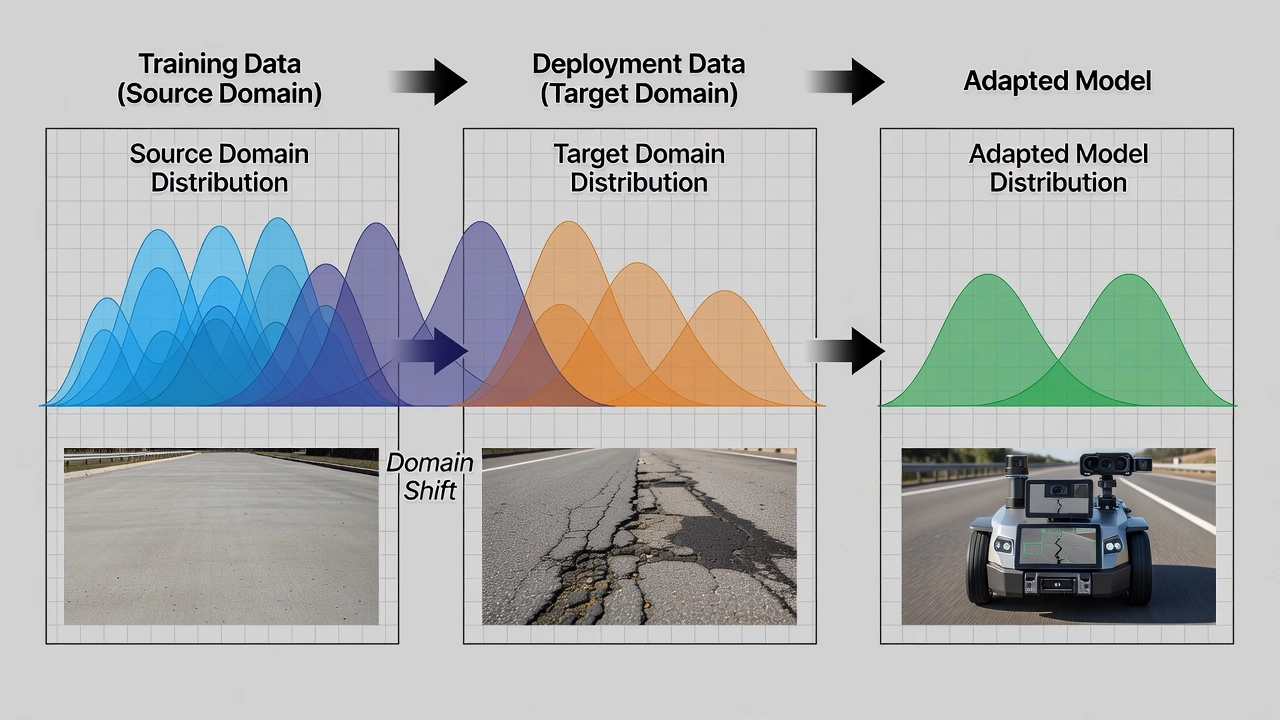
\includegraphics[width=260mm,height=104mm,keepaspectratio]{assets/referencias_visuales/tarmac_domain.png}\par
\vspace{2mm}
{\fontsize{18}{24}\selectfont Simulador \(\rightarrow\) HUCA\par}
\credit{\href{https://www.tarmacview.com/es/glossary/domain-adaptation/}{Fuente de la ilustración: TarmacView, glosario de adaptación de dominio.}}
\note{El esquema de TarmacView utiliza la inspección de pavimentos para ilustrar el cambio entre los datos de entrenamiento y los de aplicación. En ECG, Gliner y colaboradores estudiaron un cambio parecido al pasar de trazados escaneados a fotos de móvil. En este TFG, el origen es el simulador y el destino son los registros del HUCA. La adaptación intenta reducir el efecto de ese cambio sobre el modelo.}
\end{frame}}

\expandafter\newcommand\csname Slidep05\endcsname{%
\renewcommand{\defenseblock}{Datos y simulación}
\renewcommand{\defensenav}{Defensa del TFG}
\begin{frame}[t]\hypertarget{p05}{}
\frametitle{Conjuntos de datos del simulador y del HUCA}
\centering
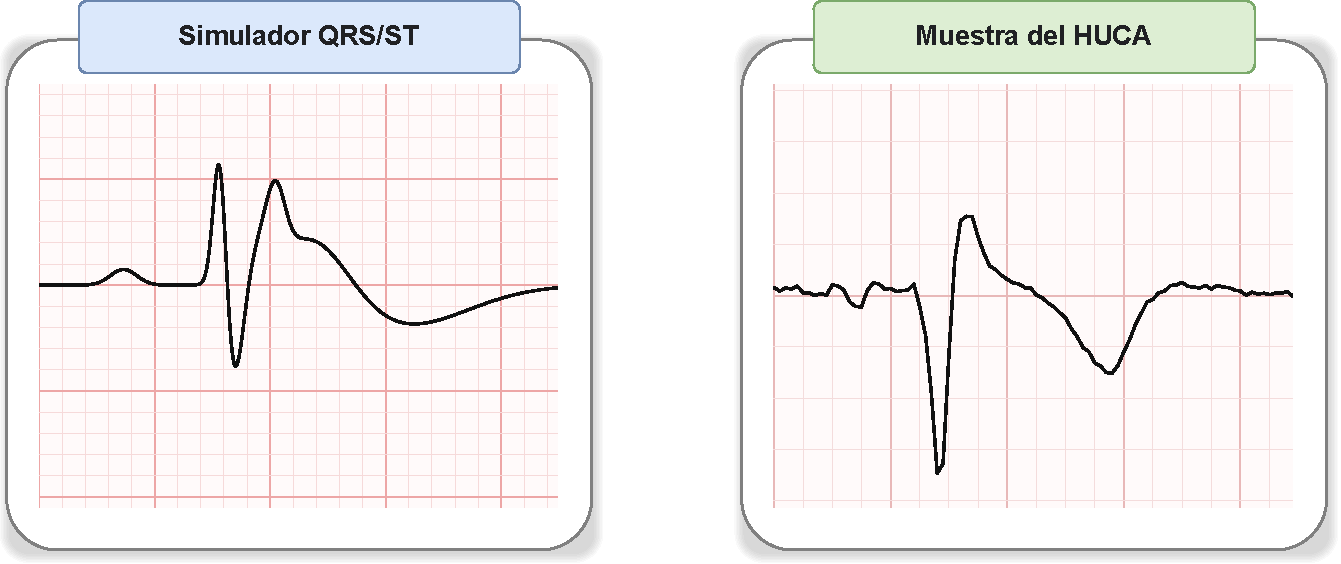
\includegraphics[width=262mm,height=111mm,keepaspectratio]{assets/fig_synthetic_real_comparison.pdf}\par
\vspace{3mm}
\begin{minipage}{262mm}\centering
\makebox[.49\linewidth]{\fontsize{22}{30}\selectfont\SimPatients{} casos, \SimPositive{} positivos}%
\makebox[.49\linewidth]{\fontsize{22}{30}\selectfont\HucaPatients{} pacientes, \HucaPositive{} positivos}
\end{minipage}
\note{Los dos conjuntos aportan imágenes de un latido de V1. El simulador genera \SimPatients{} casos y sus etiquetas describen rasgos morfológicos. El HUCA aporta \HucaPatients{} pacientes con una etiqueta clínica por persona. Los trazados que se muestran son ejemplos independientes.}
\end{frame}}

\expandafter\newcommand\csname Slidep06\endcsname{%
\renewcommand{\defenseblock}{Datos y simulación}
\renewcommand{\defensenav}{Defensa del TFG}
\begin{frame}[t]\hypertarget{p06}{}
\frametitle{Simulador QRS/ST}
\fullfigure[109mm]{gaussian_generator.drawio.pdf}
\takeaway{El latido se construye como suma de gaussianas.}
\note{El simulador construye cada latido sumando gaussianas. Su amplitud, posición y anchura permiten modificar regiones de las ondas. Sayadi y colaboradores utilizaron componentes gaussianos en un modelo dinámico. El simulador de este trabajo suma directamente los componentes. Las etiquetas se asignan a partir de los rasgos que aparecen en el latido generado.}
\end{frame}}

\expandafter\newcommand\csname Slidea04\endcsname{%
\renewcommand{\defenseblock}{Datos y simulación}
\renewcommand{\defensenav}{Defensa del TFG}
\begin{frame}[t]\hypertarget{a04}{}
\frametitle{Familias del simulador}
\fullfigure[123mm]{fig_synthetic_examples.pdf}
\note{Las familias incluyen un trazado de referencia y distintas combinaciones de cambios en el QRS, el ST y la onda T. Cada familia permite generar ejemplos con una morfología distinta.}
\end{frame}}

\expandafter\newcommand\csname Slidea05\endcsname{%
\renewcommand{\defenseblock}{Datos y simulación}
\renewcommand{\defensenav}{Defensa del TFG}
\begin{frame}[t]\hypertarget{a05}{}
\frametitle{Distribución de etiquetas en el simulador}
\fullfigure[123mm]{fig_label_distribution.pdf}
\note{Los rasgos morfológicos pueden coexistir. La regla que exige los tres produce \SimPositive{} positivos y \SimNegative{} negativos entre los \SimPatients{} casos simulados. Este desequilibrio motiva el uso de métricas que describan el rendimiento en ambas clases y en la clase positiva.}
\end{frame}}

\expandafter\newcommand\csname Slidehuca\endcsname{%
\renewcommand{\defenseblock}{Datos y simulación}
\renewcommand{\defensenav}{Defensa del TFG}
\begin{frame}[t]\hypertarget{huca}{}
\frametitle{Conjunto clínico del HUCA}
\begin{columns}[c,onlytextwidth]
\begin{column}{.55\textwidth}
\centering
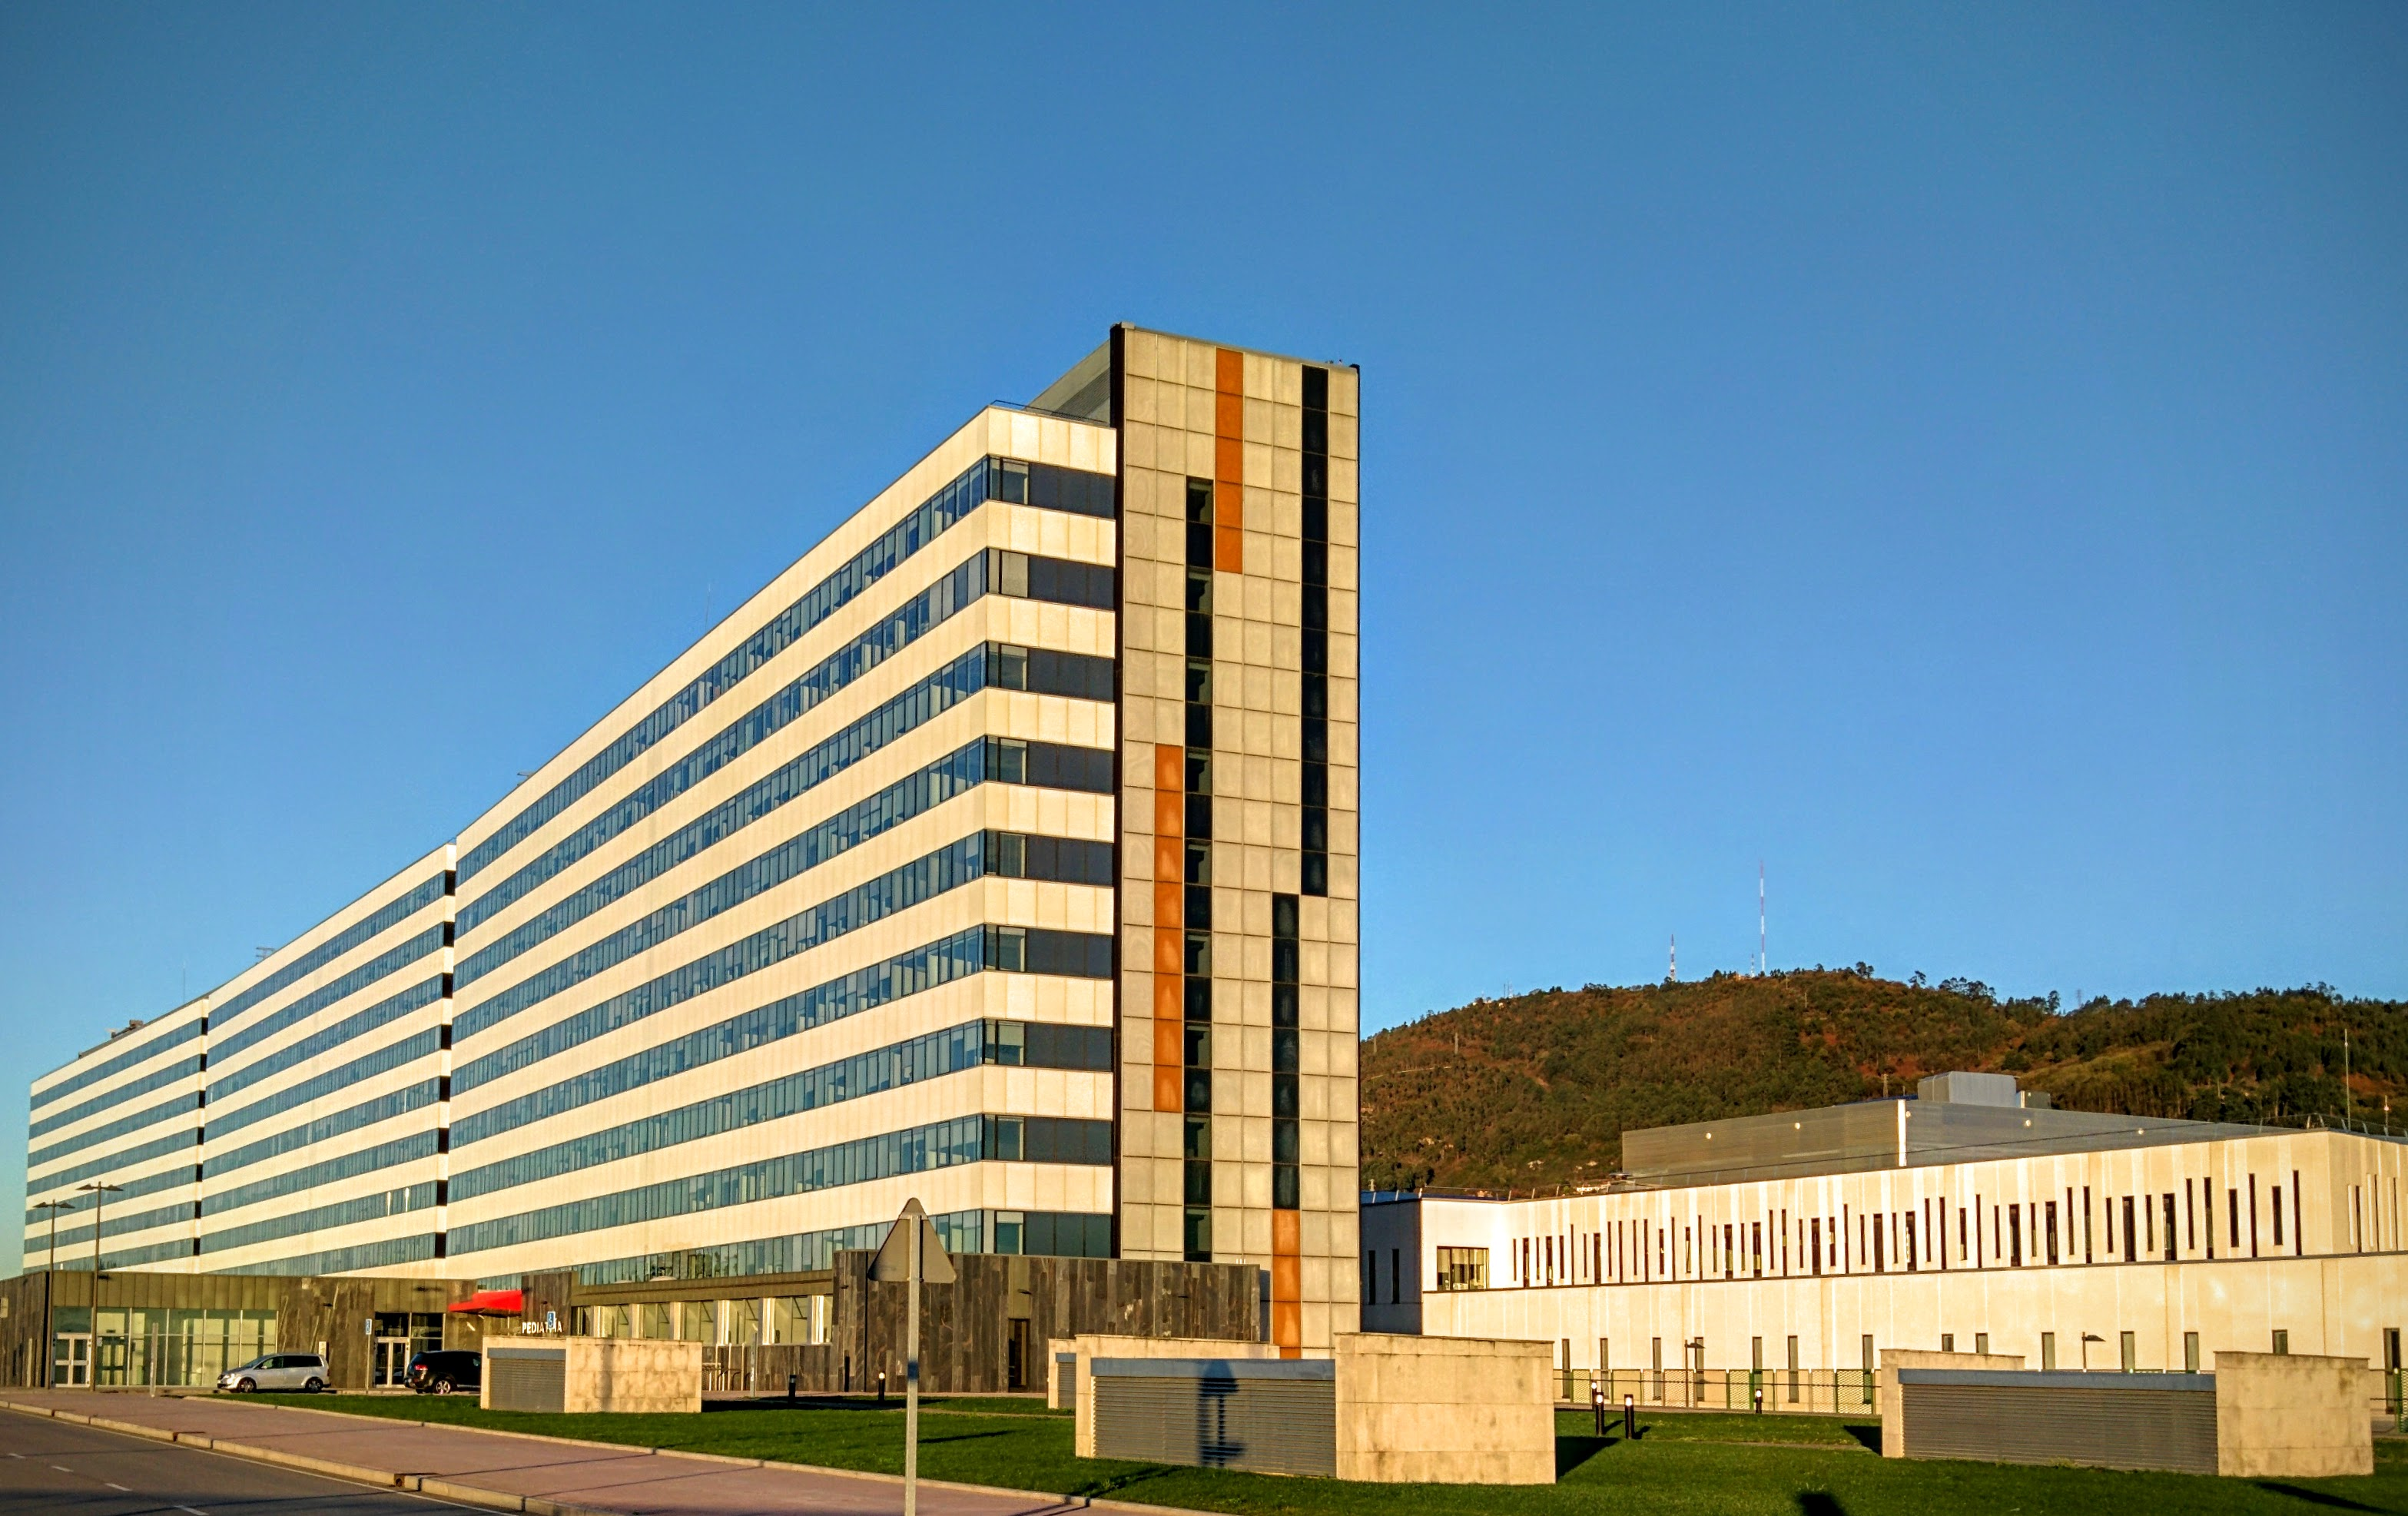
\includegraphics[width=\linewidth,height=100mm,keepaspectratio]{assets/referencias_visuales/huca.jpg}\par
\credit{\href{https://commons.wikimedia.org/wiki/File:HUCA.jpg}{Hospital Universitario Central de Asturias. LMLM, Wikimedia Commons (CC BY-SA 4.0).}}
\end{column}
\begin{column}{.41\textwidth}
{\color{UOGreen}\fontsize{45}{52}\selectfont\HucaPatients{}}\enspace{\fontsize{23}{30}\selectfont pacientes}\par
\vspace{4mm}
{\fontsize{19}{26}\selectfont\HucaPositive{} con etiqueta positiva\par
\HucaNegative{} con etiqueta negativa\par}
\vspace{8mm}
{\color{UOGreen}\fontsize{23}{30}\selectfont Selección de casos\par}
{\fontsize{19}{26}\selectfont Se excluyeron 46 casos dudosos.\par}
\end{column}
\end{columns}
\note{La campaña evaluó \HucaPatients{} pacientes, con \HucaPositive{} etiquetas positivas y \HucaNegative{} negativas. Según la memoria, se excluyeron casos que los colaboradores clínicos aconsejaron dejar fuera por dudas de clasificación. En el código, los 46 casos excluidos son los que tenían a la vez la etiqueta positiva de Brugada y el indicador de patrón basal patológico en la copia de trabajo. La copia pública de PhysioNet tiene etiquetas distintas. Los recuentos de la diapositiva corresponden a la muestra utilizada en el TFG.}
\end{frame}}

\expandafter\newcommand\csname Slidep04\endcsname{%
\renewcommand{\defenseblock}{Diseño experimental}
\renewcommand{\defensenav}{Defensa del TFG}
\begin{frame}[t]\hypertarget{p04}{}
\frametitle{Diseño experimental}
\vspace{3mm}\fullfigure[123mm]{fig_pipeline_experimental.pdf}
\note{El esquema reúne dos formas de utilizar las mismas entradas. La CNN ajusta sus pesos con imágenes etiquetadas. Gemma utiliza demostraciones dentro de la consulta. Los dos enfoques se comparan en el simulador, en transferencia a registros clínicos y con ejemplos del HUCA.}
\end{frame}}

\expandafter\newcommand\csname Slidep07\endcsname{%
\renewcommand{\defenseblock}{Implementación}
\renewcommand{\defensenav}{Defensa del TFG}
\begin{frame}[t]\hypertarget{p07}{}
\frametitle{Implementación de la CNN con ResNet18}
\vspace{3mm}\fullfigure[123mm]{cnn_convolutional_pipeline.pdf}
\note{La CNN utiliza ResNet18 preentrenada y ajusta la red completa. La imagen se convierte a gris, se redimensiona y se replica su intensidad en tres canales para respetar la entrada de ResNet18. El simulador requiere tres salidas morfológicas. El entrenamiento con HUCA utiliza una salida para la etiqueta clínica.}
\end{frame}}

\expandafter\newcommand\csname Slidea06\endcsname{%
\renewcommand{\defenseblock}{Implementación}
\renewcommand{\defensenav}{Defensa del TFG}
\begin{frame}[t]\hypertarget{a06}{}
\frametitle{Inspección de activaciones con Grad-CAM}
\vspace{3mm}\fullfigure[123mm]{cnn_simulator_qrs_gradcam_example.pdf}
\note{Grad-CAM permite inspeccionar qué regiones de la imagen se asocian con una salida de la CNN. Aquí se muestra la salida correspondiente al rasgo RBBB mediante la imagen, el mapa de activación y su superposición. El análisis es cualitativo. El mapa muestra una asociación con la salida del modelo.}
\end{frame}}

\expandafter\newcommand\csname Slidep08\endcsname{%
\renewcommand{\defenseblock}{Implementación}
\renewcommand{\defensenav}{Defensa del TFG}
\begin{frame}[t]\hypertarget{p08}{}
\frametitle{Implementación del ICL con Gemma 4 E4B}
\vspace{3mm}\fullfigure[123mm]{vlm_icl_context_window.pdf}
\note{E4B es una variante compacta de la familia Gemma 4 de Google. La consulta contiene instrucciones, demostraciones etiquetadas y la imagen que se quiere clasificar. Se prueban selecciones estándar y balanceadas por clase. El modelo devuelve etiquetas estructuradas para calcular las métricas.}
\end{frame}}

\expandafter\newcommand\csname Slideescenarios\endcsname{%
\renewcommand{\defenseblock}{Diseño experimental}
\renewcommand{\defensenav}{Defensa del TFG}
\begin{frame}[t]\hypertarget{escenarios}{}
\frametitle{Escenarios de evaluación}
\vspace{11mm}\centering
{\fontsize{22}{30}\selectfont
\setlength{\tabcolsep}{6mm}
\renewcommand{\arraystretch}{1.55}
\begin{tabular}{@{}p{102mm}p{74mm}p{63mm}@{}}
\toprule
\scenarioheading
\midrule
\hyperlink{escenario_simulador}{\textcolor{UOGray}{01}\enspace Simulación} & Simulador & Simulador\\
\hyperlink{escenario_transferencia}{\textcolor{UOGray}{02}\enspace Cambio de dominio} & Simulador & HUCA\\
\hyperlink{escenario_clinico}{\textcolor{UOGray}{03}\enspace Evaluación clínica} & HUCA & HUCA\\
\bottomrule
\end{tabular}\par}
\note{Primero se evalúan los dos enfoques dentro del simulador. Después se mantienen los ejemplos simulados y se pasa a evaluar en el HUCA, donde también se prueban estrategias de adaptación. Por último, tanto los ejemplos como la evaluación proceden del HUCA.}
\end{frame}}

\expandafter\newcommand\csname Slidep09\endcsname{%
\renewcommand{\defenseblock}{Diseño experimental}
\renewcommand{\defensenav}{Defensa del TFG}
\begin{frame}[t]\hypertarget{p09}{}
\frametitle{Protocolo de evaluación por paciente: LOOCV}
\vspace{3mm}\fullfigure[123mm]{clinical_fold_protocol.pdf}
\note{K es el número de casos de entrenamiento o demostraciones. Se evalúan cinco valores con tres semillas. Cada pliegue reserva un paciente para la prueba. La CNN clínica dispone además de ocho pacientes de validación para elegir época y umbral. La exactitud balanceada promedia sensibilidad y especificidad. F1 combina precisión y sensibilidad de la clase positiva.}
\end{frame}}

\expandafter\newcommand\csname Slideescenario_simulador\endcsname{%
\renewcommand{\defenseblock}{Resultados}
\renewcommand{\defensenav}{Defensa del TFG}
\begin{frame}[plain]\hypertarget{escenario_simulador}{}
\scenariofocus{Simulación}{Simulador}{Simulador}
\note{En el primer escenario, los ejemplos y los datos de prueba son simulados.}
\end{frame}}

\expandafter\newcommand\csname Slidep10\endcsname{%
\renewcommand{\defenseblock}{Resultados 1/3 \enspace Simulador \(\rightarrow\) Simulador}
\renewcommand{\defensenav}{Defensa del TFG}
\begin{frame}[t]\hypertarget{p10}{}
\frametitle{Entrenamiento y evaluación con datos simulados}
\vspace{6mm}
\twopictures{comparison_simulator_ba_by_k.pdf}{comparison_simulator_f1_by_k.pdf}
\note{En este escenario, tanto los ejemplos como la prueba proceden del simulador. La CNN se entrena con esos casos y Gemma los utiliza como demostraciones. El eje horizontal indica cuántos ejemplos recibe cada enfoque. A la izquierda se muestra la exactitud balanceada y a la derecha, F1. Las dos curvas muestran una mejora al aumentar la cantidad de ejemplos. Con treinta y dos, la exactitud balanceada es \SimCnnBA{} para la CNN y \SimVlmBA{} para Gemma con selección balanceada. Las barras indican variación entre semillas. El resultado describe el reconocimiento de las reglas morfológicas del simulador.}
\end{frame}}

\expandafter\newcommand\csname Slidea07\endcsname{%
\renewcommand{\defenseblock}{Resultados 1/3 \enspace Simulador \(\rightarrow\) Simulador}
\renewcommand{\defensenav}{Defensa del TFG}
\begin{frame}[t]\hypertarget{a07}{}
\frametitle{Matrices de confusión en el simulador}
\vspace{6mm}
\twopictures{cnn_simulator_qrs_k32_confusion_matrix.pdf}{vlm_simulator_qrs_balanced_k32_confusion_matrix.pdf}
\note{Las matrices comparan CNN y Gemma con treinta y dos ejemplos. Cada una agrega tres evaluaciones de los mismos casos. Gemma con selección balanceada produce menos falsos positivos en esta configuración. La matriz permite distinguir ese efecto de los errores sobre la clase positiva.}
\end{frame}}

\expandafter\newcommand\csname Slideescenario_transferencia\endcsname{%
\renewcommand{\defenseblock}{Resultados}
\renewcommand{\defensenav}{Defensa del TFG}
\begin{frame}[plain]\hypertarget{escenario_transferencia}{}
\scenariofocus{Cambio de dominio}{Simulador}{HUCA}
\note{En el segundo escenario se mantienen los ejemplos simulados y se evalúa en el HUCA.}
\end{frame}}

\expandafter\newcommand\csname Slidep11\endcsname{%
\renewcommand{\defenseblock}{Resultados 2/3 \enspace Simulador \(\rightarrow\) HUCA}
\renewcommand{\defensenav}{Defensa del TFG}
\begin{frame}[t]\hypertarget{p11}{}
\frametitle{CNN entrenada en el simulador y evaluada en el HUCA}
\vspace{3mm}\fullfigure[123mm]{domain_gap_cnn_ba_by_k.pdf}
\note{Aquí se entrena la CNN con datos del simulador y se cambia el conjunto de prueba. La línea continua representa la evaluación simulada y la discontinua, la clínica. Con treinta y dos ejemplos la exactitud balanceada clínica queda en \TransferCnnLastBA{}. El cambio de dominio afecta tanto al aspecto del trazado como a las etiquetas.}
\end{frame}}

\expandafter\newcommand\csname Slidea09\endcsname{%
\renewcommand{\defenseblock}{Resultados 2/3 \enspace Simulador \(\rightarrow\) HUCA}
\renewcommand{\defensenav}{Defensa del TFG}
\begin{frame}[t]\hypertarget{a09}{}
\frametitle{Métodos de adaptación de dominio en la CNN}
\centering
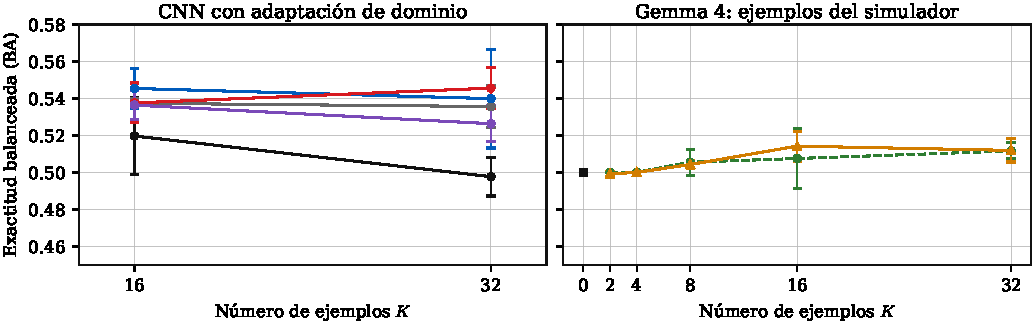
\includegraphics[width=257mm]{assets/transfer_ba.pdf}\par

\includegraphics[width=257mm]{assets/transfer_legend.pdf}\par
\note{Las variantes de adaptación incorporan imágenes clínicas sin etiqueta, incluidas las que luego se evalúan. Las etiquetas de entrenamiento siguen procediendo del simulador. CORAL y MMD mejoran algunos puntos frente a la CNN base con el mismo K. El mejor resultado global sigue correspondiendo a la CNN sin adaptación. El panel derecho muestra el resultado de Gemma con ejemplos simulados.}
\end{frame}}

\expandafter\newcommand\csname Slidea10\endcsname{%
\renewcommand{\defenseblock}{Resultados 2/3 \enspace Simulador \(\rightarrow\) HUCA}
\renewcommand{\defensenav}{Defensa del TFG}
\begin{frame}[t]\hypertarget{a10}{}
\frametitle{F1 de la clase positiva al cambiar de dominio}
\vspace{3mm}\fullfigure[123mm]{transfer_f1.pdf}
\note{El panel de F1 permite examinar la detección de positivos al cambiar de dominio. El rendimiento sigue siendo bajo en la clasificación clínica, tanto con las variantes de adaptación como con las demostraciones simuladas de Gemma. Esto ayuda a interpretar una especificidad alta cuando se predice casi siempre la clase negativa.}
\end{frame}}

\expandafter\newcommand\csname Slidep12\endcsname{%
\renewcommand{\defenseblock}{Resultados 2/3 \enspace Simulador \(\rightarrow\) HUCA}
\renewcommand{\defensenav}{Defensa del TFG}
\begin{frame}[t]\hypertarget{p12}{}
\frametitle{Cambio de dominio en ICL con selección balanceada}
\vspace{3mm}\fullfigure[123mm]{context_balanced.pdf}
\note{En la selección balanceada se compara qué ocurre al cambiar el origen de las demostraciones de Gemma, cuyos pesos permanecen fijos. Ante consultas clínicas, los ejemplos del HUCA ayudan a clasificar otros registros del mismo conjunto. Con demostraciones del simulador, el rendimiento clínico se mantiene próximo al azar.}
\end{frame}}

\expandafter\newcommand\csname Slidea11\endcsname{%
\renewcommand{\defenseblock}{Resultados 2/3 \enspace Simulador \(\rightarrow\) HUCA}
\renewcommand{\defensenav}{Defensa del TFG}
\begin{frame}[t]\hypertarget{a11}{}
\frametitle{Cambio de dominio en ICL con selección estándar}
\centering
\definecolor{ICLSynthetic}{HTML}{2E7D32}
\definecolor{ICLClinical}{HTML}{75B978}
\definecolor{ICLTransfer}{HTML}{666666}
{\fontsize{14}{19}\selectfont
\begin{tikzpicture}[baseline=-.5ex]\draw[ICLSynthetic,line width=1.15pt] (0,0)--(.65,0);\fill[ICLSynthetic] (.325,0) circle[radius=1.3pt];\end{tikzpicture}\enspace Simulador \quad
\begin{tikzpicture}[baseline=-.5ex]\draw[ICLClinical,dashed,line width=1.15pt] (0,0)--(.65,0);\fill[ICLClinical] (.325,0) circle[radius=1.3pt];\end{tikzpicture}\enspace HUCA, contexto HUCA \quad
\begin{tikzpicture}[baseline=-.5ex]\draw[ICLTransfer,dotted,line width=1.15pt] (0,0)--(.65,0);\fill[ICLTransfer] (.325,0) circle[radius=1.3pt];\end{tikzpicture}\enspace HUCA, contexto del simulador\par}
\vspace{3mm}
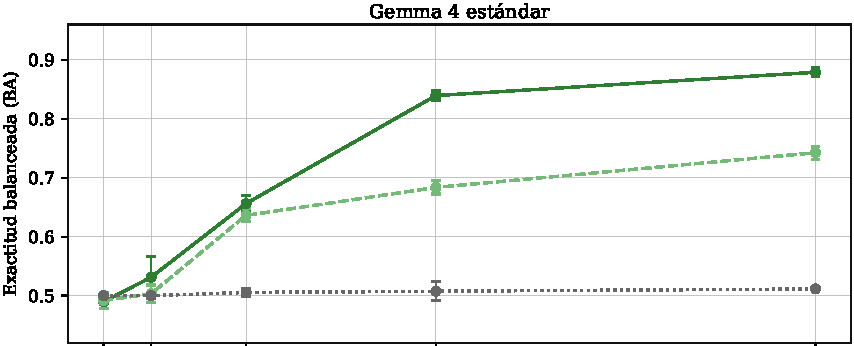
\includegraphics[width=245mm]{assets/context_standard.pdf}\par
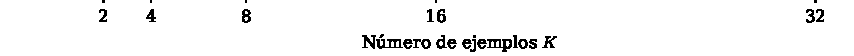
\includegraphics[width=245mm]{assets/context_xaxis.pdf}\par
\note{La selección estándar reproduce el mismo patrón general. Las consultas clínicas se benefician de ejemplos del HUCA, mientras que las demostraciones simuladas aportan poco al clasificar los registros clínicos.}
\end{frame}}

\expandafter\newcommand\csname Slideescenario_clinico\endcsname{%
\renewcommand{\defenseblock}{Resultados}
\renewcommand{\defensenav}{Defensa del TFG}
\begin{frame}[plain]\hypertarget{escenario_clinico}{}
\scenariofocus{Evaluación clínica}{HUCA}{HUCA}
\note{En el tercer escenario, tanto los ejemplos como la prueba proceden del HUCA.}
\end{frame}}

\expandafter\newcommand\csname Slidep13\endcsname{%
\renewcommand{\defenseblock}{Resultados 3/3 \enspace HUCA \(\rightarrow\) HUCA}
\renewcommand{\defensenav}{Defensa del TFG}
\begin{frame}[t]\hypertarget{p13}{}
\frametitle{Entrenamiento y demostraciones con ejemplos del HUCA}
\centering

\includegraphics[width=178mm]{assets/clinical_legend.pdf}\par
\begin{columns}[T,onlytextwidth]
\begin{column}{.49\textwidth}
\centering
{\fontsize{19}{26}\selectfont Exactitud balanceada\par}
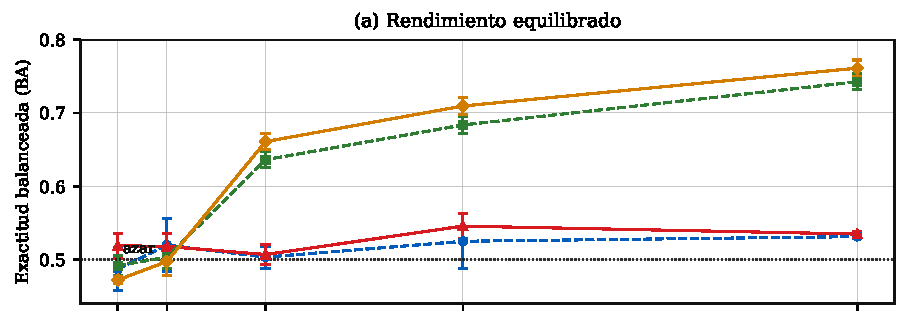
\includegraphics[width=\linewidth,trim=0 0 0 15bp,clip]{assets/clinical_ba.pdf}\par
\vspace{-1mm}
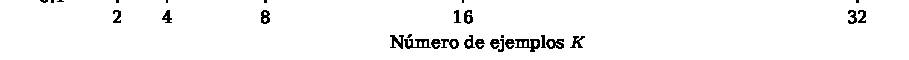
\includegraphics[width=\linewidth,trim=0 0 0 3bp,clip]{assets/clinical_xaxis.pdf}\par
\end{column}
\begin{column}{.49\textwidth}
\centering
{\fontsize{19}{26}\selectfont F1 de la clase positiva\par}
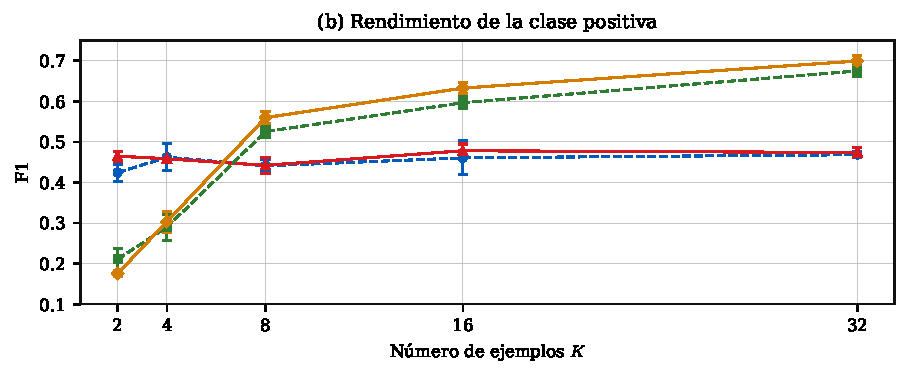
\includegraphics[width=\linewidth,trim=0 0 0 15bp,clip]{assets/clinical_f1.pdf}\par
\end{column}
\end{columns}
\takeaway{Con \(K=32\), la exactitud balanceada es \RealVlmBA{} para Gemma y \RealCnnLastBA{} para la CNN en selección balanceada.}
\note{En el tercer escenario, la CNN se entrena directamente con imágenes del HUCA y Gemma recibe demostraciones del mismo conjunto. El paciente de prueba queda reservado en ambos casos. A la izquierda vemos la exactitud balanceada. A la derecha se muestra F1 para la clase positiva. F1 baja cuando el modelo deja casos positivos sin detectar o cuando da demasiadas falsas alarmas. Sin demostraciones, Gemma no resulta capaz de identificar positivos en la evaluación realizada. Con dos o cuatro ejemplos, la mejor CNN conserva una ligera ventaja. Desde ocho ejemplos, Gemma con selección balanceada obtiene mejores resultados. Con treinta y dos alcanza una exactitud balanceada de \RealVlmBA{}, frente a \RealCnnLastBA{} de la CNN balanceada, y un F1 de \RealVlmFone{}. La comparación se refiere a esta muestra y a las configuraciones evaluadas.}
\end{frame}}

\expandafter\newcommand\csname Slidep14\endcsname{%
\renewcommand{\defenseblock}{Resultados 3/3 \enspace HUCA \(\rightarrow\) HUCA}
\renewcommand{\defensenav}{Defensa del TFG}
\begin{frame}[t]\hypertarget{p14}{}
\frametitle{Matrices de confusión en la evaluación clínica}
\vspace{3mm}\fullfigure[123mm]{clinical_cnn_vs_gemma_confusions.pdf}
\note{Las matrices muestran las mejores configuraciones balanceadas de cada método. La CNN utiliza dieciséis ejemplos y Gemma, treinta y dos. Gemma obtiene una sensibilidad de \RealVlmSens{} y una especificidad de \RealVlmSpec{}. Esto deja sin identificar alrededor de una cuarta parte de los positivos. Las matrices se normalizan por clase real y agregan tres evaluaciones de los mismos pacientes.}
\end{frame}}

\expandafter\newcommand\csname Slidea15\endcsname{%
\renewcommand{\defenseblock}{Discusión y conclusiones}
\renewcommand{\defensenav}{Defensa del TFG}
\begin{frame}[t]\hypertarget{a15}{}
\frametitle{Aspectos éticos y protección de datos}
\vspace{14mm}
\begin{columns}[t,onlytextwidth]
\begin{column}{.46\textwidth}
{\color{UOGreen}\rule{\linewidth}{1pt}}\par\vspace{5mm}
{\fontsize{26}{33}\selectfont Protección de los datos\par}
\vspace{6mm}
{\fontsize{20}{28}\selectfont Modelos de pesos abiertos para procesar los ECG sin enviarlos a servicios externos.\par}
\end{column}
\begin{column}{.46\textwidth}
{\color{UOGreen}\rule{\linewidth}{1pt}}\par\vspace{5mm}
{\fontsize{26}{33}\selectfont Responsabilidad clínica\par}
\vspace{6mm}
{\fontsize{20}{28}\selectfont Apoyo al triaje ante sospecha de síndrome de Brugada.\par}
\end{column}
\end{columns}
\note{El HUCA entregó los registros anonimizados. Los pesos abiertos de Gemma 4 permitieron ejecutar la inferencia en un clúster privado, sin enviar ECG a un servicio externo. La aplicación que se plantea es el apoyo al triaje: ordenar qué ECG revisar primero bajo responsabilidad del personal sanitario.}
\end{frame}}

\expandafter\newcommand\csname Slidep15\endcsname{%
\renewcommand{\defenseblock}{Discusión y conclusiones}
\renewcommand{\defensenav}{Defensa del TFG}
\begin{frame}[t]\hypertarget{p15}{}
\frametitle{Discusión y limitaciones}
\vspace{22mm}
\begin{columns}[T,onlytextwidth]
\begin{column}{.22\textwidth}\centering
{\color{UOGreen}\fontsize{22}{29}\selectfont Un centro\par}
\vspace{3mm}
{\fontsize{17}{23}\selectfont HUCA\par}
\end{column}
\begin{column}{.26\textwidth}\centering
{\color{UOGreen}\fontsize{22}{29}\selectfont Etiquetas distintas\par}
\vspace{3mm}
{\fontsize{17}{23}\selectfont Rasgos morfológicos\\y etiqueta clínica\par}
\end{column}
\begin{column}{.22\textwidth}\centering
{\color{UOGreen}\fontsize{22}{29}\selectfont Un latido\par}
\vspace{3mm}
{\fontsize{17}{23}\selectfont Derivación precordial V1\par}
\end{column}
\begin{column}{.27\textwidth}\centering
{\color{UOGreen}\fontsize{22}{29}\selectfont Modelos open-weight\par}
\vspace{3mm}
{\fontsize{17}{23}\selectfont Privacidad de los pacientes\par}
\end{column}
\end{columns}
\note{Los ECG proceden de un solo centro, el HUCA. El simulador etiqueta rasgos morfológicos y los datos clínicos aportan una etiqueta por paciente. La entrada se limita a un latido de la derivación precordial V1. Elegimos un modelo de pesos abiertos para ejecutar la inferencia en nuestro entorno y evitar enviar los ECG a servicios externos. En ECGBench, algunos modelos cerrados superaron a varios modelos abiertos de propósito general en ciertas tareas. El rendimiento depende del modelo y de la tarea, y PULSE, un modelo abierto especializado en ECG, superó a los modelos cerrados evaluados en varias tareas. \href{https://aimedlab.github.io/PULSE/}{Liu y colaboradores (2026).}}
\end{frame}}

\expandafter\newcommand\csname Slidep16\endcsname{%
\renewcommand{\defenseblock}{Discusión y conclusiones}
\renewcommand{\defensenav}{Defensa del TFG}
\begin{frame}[t]\hypertarget{p16}{}
\frametitle{Conclusiones}
\vspace{8mm}
\begin{columns}[t,onlytextwidth]
\begin{column}{.31\textwidth}
{\color{UOGreen}\rule{\linewidth}{1.15pt}}\par\vspace{4mm}
{\fontsize{22}{29}\selectfont Número de ejemplos\par}
\vspace{9mm}
{\color{UOGreen}\fontsize{32}{43}\selectfont Mejora en ambos\par}
\vspace{3mm}
{\fontsize{18}{26}\selectfont En el simulador, ambos métodos mejoran al disponer de más ejemplos etiquetados.\par}
\end{column}
\begin{column}{.31\textwidth}
{\color{UOGreen}\rule{\linewidth}{1.15pt}}\par\vspace{4mm}
{\fontsize{22}{29}\selectfont Comparación en el HUCA\par}
\vspace{9mm}
\begin{minipage}[t]{.48\linewidth}
{\color{UOGreen}\fontsize{35}{43}\selectfont\strut\RealVlmBA{}\par}
{\fontsize{17}{22}\selectfont Gemma\par}
\end{minipage}\hfill
\begin{minipage}[t]{.48\linewidth}
{\color{UOGreen}\fontsize{35}{43}\selectfont\strut\RealCnnLastBA{}\par}
{\fontsize{17}{22}\selectfont CNN\par}
\end{minipage}\par\vspace{3mm}
{\fontsize{18}{26}\selectfont Exactitud balanceada con 32 ejemplos del HUCA y selección balanceada.\par}
\end{column}
\begin{column}{.31\textwidth}
{\color{UOGreen}\rule{\linewidth}{1.15pt}}\par\vspace{4mm}
{\fontsize{22}{29}\selectfont Transferencia al HUCA\par}
\vspace{9mm}
{\color{UOGreen}\fontsize{35}{43}\selectfont\TransferCnnLastBA{}\par}
\vspace{3mm}
{\fontsize{18}{26}\selectfont Exactitud balanceada en el HUCA de la CNN entrenada con 32 ejemplos simulados.\par}
\end{column}
\end{columns}
\note{Aumentar el número de ejemplos mejora el rendimiento de ambos métodos en la tarea simulada. En el HUCA, Gemma con selección balanceada supera a la CNN a partir de ocho ejemplos. Con 32 ejemplos, sus exactitudes balanceadas son \RealVlmBA{} y \RealCnnLastBA{}, respectivamente. Al entrenar la CNN con 32 ejemplos simulados y evaluarla en el HUCA, el resultado queda en \TransferCnnLastBA{}, cerca del azar.}
\end{frame}}

\expandafter\newcommand\csname Slidefuturo\endcsname{%
\renewcommand{\defenseblock}{Discusión y conclusiones}
\renewcommand{\defensenav}{Defensa del TFG}
\begin{frame}[t]\hypertarget{futuro}{}
\frametitle{Continuación del trabajo}
\vspace{12mm}
{\fontsize{23}{31}\selectfont
\begin{tabular}{@{}p{17mm}l@{}}
\textcolor{UOGreen}{01} & Revisar las etiquetas y ampliar su recogida\\[7mm]
\textcolor{UOGreen}{02} & Explorar otros rasgos morfológicos del ECG\\[7mm]
\textcolor{UOGreen}{03} & Explorar otros métodos de adaptación de dominio\\[7mm]
\textcolor{UOGreen}{04} & Validar el apoyo al triaje en el HUCA y después en otros centros
\end{tabular}}
\note{La continuación empieza por revisar las etiquetas con especialistas y ampliar la recogida de casos etiquetados. Se estudiarían otros rasgos morfológicos del ECG y se probarían otros métodos de adaptación de dominio. Por último, se evaluaría si el sistema ayuda a priorizar ECG sospechosos en el HUCA y después en otros centros sanitarios.}
\end{frame}}

\expandafter\newcommand\csname Slidecierre\endcsname{%
\renewcommand{\defenseblock}{}
\renewcommand{\defensenav}{Defensa del TFG}
\begin{frame}[plain]\hypertarget{cierre}{}
\hypertarget{conclusion}{}
\centering
\vspace*{5mm}

\includegraphics[height=33mm]{assets/logo_uniovi_portada.pdf}\par
\vspace{6mm}
{\fontsize{32}{40}\selectfont Gracias por su atención\par}
\vspace{7mm}
{\fontsize{19}{25}\selectfont Preguntas\par}
\vspace{6mm}
{\fontsize{21}{27}\selectfont\AuthorName\par}
{\fontsize{17}{23}\selectfont \hyperlink{a13}{Referencias}\par}
\vfill

\includegraphics[height=9mm]{assets/logo_epi_horizontal.pdf}\hfill
{\fontsize{17}{22}\selectfont\SubmissionDate}\par
\note{Gracias por su atención. Quedo a disposición del tribunal para las preguntas.}
\end{frame}}

\expandafter\newcommand\csname Slidea13\endcsname{%
\renewcommand{\defenseblock}{Referencias}
\renewcommand{\defensenav}{\hyperlink{a14}{Métodos y métricas}\quad \hyperlink{conclusion}{Volver al cierre}}
\begin{frame}[t]\hypertarget{a13}{}
\frametitle{Referencias clínicas y estado del arte}
\vspace{5mm}
\begin{columns}[T,onlytextwidth]
\begin{column}{.48\textwidth}
{\fontsize{22}{29}\selectfont\color{UOGreen} Contexto clínico y datos\par}
\vspace{4mm}
{\fontsize{16}{22}\selectfont\raggedright
\href{https://www.who.int/en/news-room/fact-sheets/detail/cardiovascular-diseases-(cvds)}{OMS. Mortalidad cardiovascular mundial.}\par\vspace{2mm}
\href{https://doi.org/10.1093/eurheartj/ehac262}{Zeppenfeld et al. (2022). Guías ESC y Brugada.}\par\vspace{2mm}
\href{https://doi.org/10.1161/CIRCULATIONAHA.106.180200}{Kligfield et al. (2007). ECG de doce derivaciones.}\par\vspace{2mm}
\href{https://doi.org/10.1161/CIRCULATIONAHA.108.191095}{Surawicz et al. (2009). Bloqueos de rama.}\par\vspace{2mm}
\href{https://physionet.org/content/brugada-huca/1.0.0/}{Costa Cortez y García Iglesias (2026). Brugada-HUCA.}\par\vspace{2mm}
\href{https://doi.org/10.1038/s41597-020-0495-6}{Wagner et al. (2020). Conjunto PTB-XL.}\par\vspace{2mm}
\href{https://commons.wikimedia.org/wiki/File:Brugada_syndrome_type1_example4_(CardioNetworks_ECGpedia).png}{ECGpedia} y \href{https://doi.org/10.1186/1750-1172-1-35}{Napolitano y Priori (2006). Ejemplos de patrones de Brugada.}\par}
\end{column}
\begin{column}{.48\textwidth}
{\fontsize{22}{29}\selectfont\color{UOGreen} Antecedentes\par}
\vspace{4mm}
{\fontsize{16}{22}\selectfont\raggedright
\href{https://pmc.ncbi.nlm.nih.gov/articles/PMC7145824/}{Ribeiro et al. (2020). Clasificación de señales de ECG.}\par\vspace{2mm}
\href{https://pmc.ncbi.nlm.nih.gov/articles/PMC8948243/}{Sangha et al. (2022). Clasificación de imágenes de ECG.}\par\vspace{2mm}
\href{https://pmc.ncbi.nlm.nih.gov/articles/PMC10462630/}{Gliner et al. (2023). Adaptación a fotos de ECG.}\par\vspace{2mm}
\href{https://portalinvestigacion.uniovi.es/documentos/697e9dda4f95b66d0e7b373a?lang=en}{Camba et al. (2026). ICL para imágenes de ECG.}\par\vspace{2mm}
\href{https://pubmed.ncbi.nlm.nih.gov/42330857/}{Costa et al. (2026). VLM y ECG con pocos ejemplos.}\par\vspace{2mm}
\href{https://www.tarmacview.com/es/glossary/domain-adaptation/}{TarmacView. Esquema de cambio de dominio.}\par}
\end{column}
\end{columns}
\note{Las referencias de contexto respaldan la motivación clínica y la procedencia de los datos y trazados. Los antecedentes corresponden al análisis de señales, el análisis de imágenes, el cambio de dominio y el aprendizaje con pocos ejemplos. Los créditos y las licencias de las imágenes publicadas se detallan en el proyecto LaTeX.}
\end{frame}}

\expandafter\newcommand\csname Slidea14\endcsname{%
\renewcommand{\defenseblock}{Referencias}
\renewcommand{\defensenav}{\hyperlink{a13}{Clínica y antecedentes}\quad \hyperlink{conclusion}{Volver al cierre}}
\begin{frame}[t]\hypertarget{a14}{}
\frametitle{Referencias de métodos y métricas}
\vspace{5mm}
\begin{columns}[T,onlytextwidth]
\begin{column}{.48\textwidth}
{\fontsize{22}{29}\selectfont\color{UOGreen} Simulador y modelos\par}
\vspace{4mm}
{\fontsize{16}{22}\selectfont\raggedright
\href{https://pmc.ncbi.nlm.nih.gov/articles/PMC3148951/}{Sayadi et al. (2010). Generación de ECG con gaussianas.}\par\vspace{2mm}
\href{https://openaccess.thecvf.com/content_cvpr_2016/html/He_Deep_Residual_Learning_CVPR_2016_paper.html}{He et al. (2016). Redes residuales.}\par\vspace{2mm}
\href{https://doi.org/10.1109/ICCV.2017.74}{Selvaraju et al. (2017). Grad-CAM.}\par\vspace{2mm}
\href{https://aclanthology.org/2024.emnlp-main.64/}{Dong et al. (2024). Aprendizaje en contexto.}\par\vspace{2mm}
\href{https://ai.google.dev/gemma/docs/core/model_card_4}{Google DeepMind. Ficha de Gemma 4.}\par}
\end{column}
\begin{column}{.48\textwidth}
{\fontsize{22}{29}\selectfont\color{UOGreen} Adaptación y evaluación\par}
\vspace{4mm}
{\fontsize{16}{22}\selectfont\raggedright
\href{https://proceedings.mlr.press/v119/chen20j.html}{Chen et al. (2020). SimCLR y aprendizaje contrastivo.}\par\vspace{2mm}
\href{https://arxiv.org/abs/1607.01719}{Sun y Saenko (2016). Deep CORAL.}\par\vspace{2mm}
\href{https://proceedings.mlr.press/v37/long15.html}{Long et al. (2015). Adaptación mediante MMD.}\par\vspace{2mm}
\href{https://jmlr.org/papers/v17/15-239.html}{Ganin et al. (2016). Adaptación adversarial (DANN).}\par\vspace{2mm}
\href{https://scikit-learn.org/stable/modules/generated/sklearn.metrics.f1_score.html}{Scikit-learn. Definición de F1 para la clase positiva.}\par\vspace{2mm}
\href{https://doi.org/10.1038/s41746-026-02551-3}{Liu et al. (2026). Comparación de modelos en ECGBench.}\par}
\end{column}
\end{columns}
\note{Estas fuentes identifican los métodos que aparecen en el desarrollo o los resultados, junto a la ficha del modelo y la definición de F1. Los valores experimentales proceden de los agregados canónicos del proyecto.}
\end{frame}}
